% Figura cuerpo B3: el anuncio no creíble y el sesgo inflacionista: más inflación y el mismo paro
\documentclass[tikz,border=3pt]{standalone}
\usepackage[T1]{fontenc}
\usepackage[utf8]{inputenc}
\usepackage{amsmath}
\usetikzlibrary{arrows.meta,calc,positioning}
\begin{document}
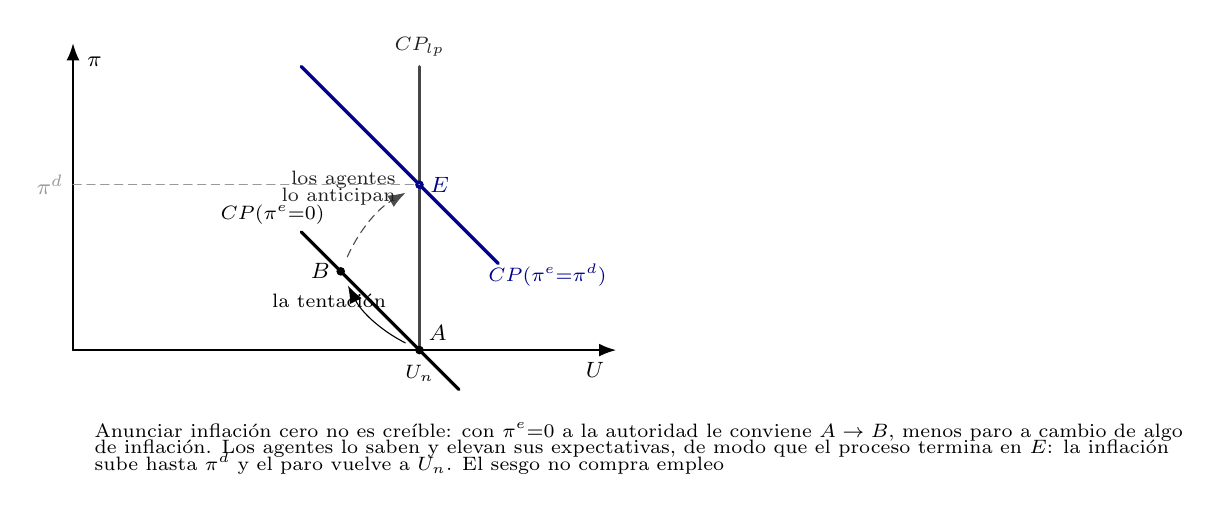
\begin{tikzpicture}[>={Latex[length=2.2mm]}, line cap=round, font=\footnotesize,
  eje/.style={->, thick},
  curva/.style={very thick},
  nueva/.style={very thick, blue!55!black},
  guia/.style={densely dashed, gray!80},
  pto/.style={circle, fill=black, inner sep=1.1pt}]
  \draw[eje] (0,0) -- (6.9,0) node[below left=1pt]{$U$};
  \draw[eje] (0,0) -- (0,3.9) node[below right=2pt]{$\pi$};
  % Phillips de largo plazo
  \draw[curva, gray!55!black] (4.4,0) -- (4.4,3.6) node[above, font=\scriptsize, text=gray!25!black]{$CP_{lp}$};
  % Curvas de corto plazo
  \draw[curva] (2.9,1.5) -- (4.9,-0.5);
  \node[anchor=west, font=\scriptsize] at (1.75,1.72) {$CP(\pi^{e}{=}0)$};
  \draw[nueva] (2.9,3.6) -- (5.4,1.1);
  \node[anchor=west, font=\scriptsize, blue!55!black] at (5.15,0.95) {$CP(\pi^{e}{=}\pi^{d})$};
  % Puntos
  \node[pto] (A) at (4.4,0) {};
  \node[inner sep=1pt] at (4.63,0.22) {$A$};
  \node[pto] (B) at (3.4,1.0) {};
  \node[left=1pt of B, inner sep=1pt] {$B$};
  \node[pto, fill=blue!55!black] (E) at (4.4,2.1) {};
  \node[right=1pt of E, inner sep=1pt, blue!55!black] {$E$};
  \draw[->, shorten >=4pt, shorten <=4pt] (A) to[bend left=18] (B);
  \node[font=\scriptsize, anchor=south east] at (4.1,0.42) {la tentación};
  \draw[->, densely dashed, gray!60!black, shorten >=4pt, shorten <=4pt] (B) to[bend left=18] (E);
  \node[font=\scriptsize, anchor=south east, text=gray!25!black, align=right] at (4.22,1.72) {los agentes\\[-2pt]lo anticipan};
  \draw[guia] (0,2.1) node[left]{$\pi^{d}$} -- (4.4,2.1);
  \node[font=\scriptsize] at (4.4,-0.3) {$U_n$};
  \node[align=left, anchor=north west, font=\scriptsize] at (0.15,-0.8)
    {Anunciar inflación cero no es creíble: con $\pi^{e}{=}0$ a la autoridad le conviene $A\to B$, menos paro a cambio de algo\\[-2pt]de inflación. Los agentes lo saben y elevan sus expectativas, de modo que el proceso termina en $E$: la inflación\\[-2pt]sube hasta $\pi^{d}$ y el paro vuelve a $U_n$. El sesgo no compra empleo};
\end{tikzpicture}
\end{document}
